% Part I, program calculation (files 01 to 04, about 20 min). For a
% general CS audience: Python first, then one switch to Haskell (02).
\partframe{Part I}{Program Calculation}

\begin{frame*}[vertical-alignment = top]
  \frametitle{Rewrite Rules You Already Trust}
  \vspace*{4mm}
  A database optimiser:
  \mainblock{sql-pushdown.sql}
  An ML compiler:
  \mainblock{torch-fusion.py}
  % Step 2: should you trust them? A real case. Step 3: a box on top.
  \only<2->{\par\nointerlineskip\vbox to 0pt{%
    \begin{tikzpicture}[overlay, remember picture, alt = {Should you really
        trust them? A real case, PyTorch issue 196468: an attention-shaped
        pattern rewrite ignores the softmax dimension, silently computing
        attention over the last axis: a fusion rule whose side condition is
        never checked.}]
      \node[anchor = north, fill = white, draw = black!25,
        rounded corners = 3pt, drop shadow, text width = 150mm,
        align = left, inner sep = 3mm]
        at ($(current page.north) + (0, -15mm)$)
        {{\Large\bfseries\color{bad} Should you really trust them?\par}\medskip
         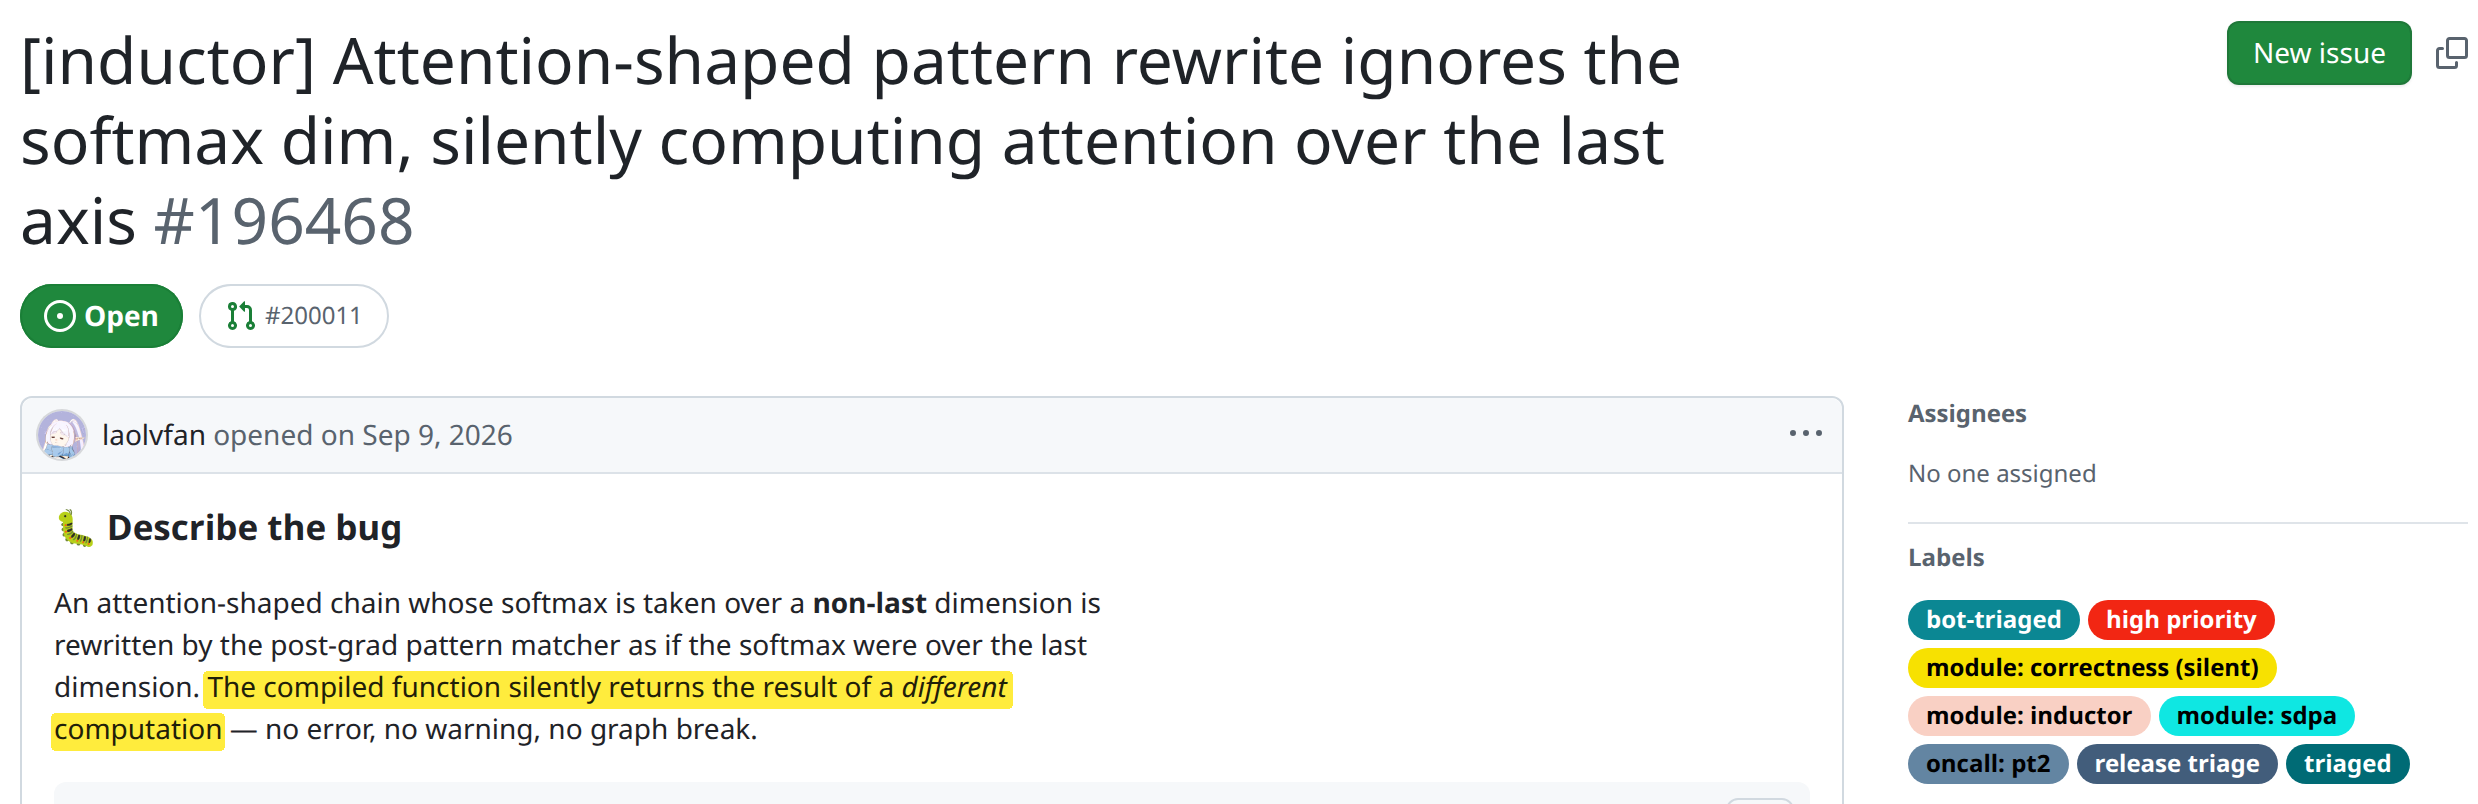
\includegraphics[width = \linewidth, alt = {Screenshot of PyTorch
          issue 196468, open, labelled high priority and correctness
          (silent)}]{pytorch-196468.png}\par\smallskip
         \small A fusion rule whose side condition (softmax over the
         \textbf{last} axis) is never checked.\par
         {\footnotesize\url{https://github.com/pytorch/pytorch/issues/196468}\par}};
    \end{tikzpicture}\vss}}
  \only<3>{\par\nointerlineskip\vbox to 0pt{%
    \begin{tikzpicture}[overlay, remember picture, alt = {To trust a
        rewrite, we need a proved law, with its side conditions checked at
        every use. Can we have that for our own programs?}]
      \node[fill = yellow!20, draw = golden!80!black, rounded corners = 3pt,
        drop shadow, text width = 130mm, align = center, inner sep = 5mm,
        font = \Large, execute at begin node = {\hyphenpenalty = 10000}]
        at ($(current page.center) + (0, -4mm)$)
        {To trust a rewrite, we need a \textbf{proved} law, with its side
        conditions \textbf{checked} at every use. Can we have that for
        \textbf{our own} programs?};
    \end{tikzpicture}\vss}}
  \speakernote{SQL: predicate pushdown, a law of relational algebra \\
    PyTorch / XLA: element-wise ops fused into one kernel \\
    Click: should you trust them? PyTorch \#196468 (open, high priority):
    the fusion ignores which axis softmax uses; a side condition nobody
    checks \\
    Click: trust needs proved laws and checked side conditions; for our own
    programs: the algebra of programming}
\end{frame*}

\begin{frame}[vertical-alignment = top]
  \frametitle{Programs as Algebra}
  \vspace*{3mm}
  Specify \emph{clearly}; \textbf{calculate} an efficient program;
  every step is an \emph{equation}.
  \par\medskip{\centering
    \begin{tikzpicture}[alt={A timeline of the algebra of programming.
        1978: Backus asks for an algebra of programs in his Turing lecture.
        1986 and 1987: Meertens and Bird, the Bird-Meertens formalism.
        1991: Meijer, Fokkinga and Paterson, recursion schemes. 1997: Bird
        and de Moor, the book Algebra of Programming. 2002: Gibbons,
        Calculating Functional Programs. 2020: Bird and Gibbons, Algorithm
        Design with Haskell.},
      ev/.style = {box, font = \footnotesize, text width = 30mm,
        align = center, execute at begin node = {\hyphenpenalty = 10000}},
      yr/.style = {font = \footnotesize\bfseries, inner sep = 1pt}]
      \draw[very thick, gray, ->] (-0.6, 0) -- (14.6, 0);
      % \s = 1: event above the line, year below; \s = -1: the other way
      % each box: who and what, then a short citation (\tlcite)
      \foreach \x/\y/\s/\t [count = \i] in {
          0.65/1978/1/{\textbf{Backus}: ``an algebra of programs''
            \tlcite{CACM 1978}},
          3.15/1986--87/-1/{\textbf{Meertens}, \textbf{Bird}: laws for
            lists \tlcite{CWI'86; NATO ASI'87}},
          5.65/1990--91/1/{\textbf{Malcolm}; \textbf{Meijer} et al.: laws
            for every data type \tlcite{SCP 1990; FPCA 1991}},
          8.15/1997/-1/{\textbf{Bird}, \textbf{de Moor}: \emph{Algebra of
            Programming} \tlcite{Prentice Hall 1997}},
          10.65/2015/1/{\textbf{Hinze}, \textbf{Wu}, \textbf{Gibbons}: one
            scheme behind them all \tlcite{POPL 2015}},
          13.15/2027/-1/{\textbf{Gibbons}: \emph{Patterns in Functional
            Programming} \tlcite{CUP, forthcoming}}} {
        \ifnum\s=1 \def\ea{south}\def\ya{north}%
        \else \def\ea{north}\def\ya{south}\fi
        \fill[accent] (\x, 0) circle (1.2mm);
        \node[yr, anchor = \ya] at (\x, -0.25 * \s) {\y};
        \node[ev, anchor = \ea] (e\i) at (\x, 0.5 * \s) {\t};
        \draw[accent] (\x, 0.12 * \s) -- (e\i);
      }
    \end{tikzpicture}\par}
  \excerpt<2>{``Conventional programming languages are growing ever more
    enormous, but not stronger. [\ldots] Associated with the functional style
    of programming is an \textbf{algebra of programs} whose variables range
    over programs and whose operations are combining forms. This algebra can
    be used to \textbf{transform programs} and to solve equations whose
    `unknowns' are programs in much the same way one transforms equations in
    high school algebra. These transformations are given by algebraic laws
    [\ldots]''}{J. Backus, Can Programming Be Liberated from the von Neumann
    Style? Turing Award lecture, CACM 21(8), 1978}
  \slideref{J. Backus. \textbf{Can Programming Be Liberated from the von Neumann Style?} CACM 1978. \rfsep
    R. Bird. \textbf{An Introduction to the Theory of Lists}. 1987. \rfsep
    G. Malcolm. \textbf{Data Structures and Program Transformation}. SCP 1990. \rfsep
    E. Meijer, M. Fokkinga, R. Paterson. \textbf{Functional Programming with Bananas, Lenses, Envelopes and Barbed Wire}. FPCA 1991. \rfsep
    R. Bird, O. de Moor. \textbf{Algebra of Programming}. Prentice Hall, 1997. \rfsep
    R. Hinze, N. Wu, J. Gibbons. \textbf{Conjugate Hylomorphisms, or: The Mother of All Structured Recursion Schemes}. POPL 2015. \rfsep
    J. Gibbons. \textbf{Patterns in Functional Programming}. CUP, forthcoming (2027).}
  \speakernote{Yes: the algebra of programming (program calculation) \\
    Backus: programs you can do algebra on \\
    Bird and Meertens: a notation and laws for lists (Squiggol) \\
    Malcolm; Meijer et al.: the same laws for every data type \\
    Bird and de Moor: the book; Hinze et al.: one scheme (hylos) \\
    Gibbons: the patterns, in a book (CUP, Feb 2027) \\
    Click: Backus's abstract (1977 Turing lecture)}
\end{frame}

\begin{frame*}
  \frametitle{A Specification and a Program}
  \mainblock{sumsq.py}
  \begin{itemize}[<+->]
    \item Equal, by a \textbf{law}: summing a mapped list is one loop
      (\emph{fusion}).
    \item Laws are proved once; the program is \textbf{correct by
      construction}.
  \end{itemize}
  \speakernote{Top: obviously right, but a temporary list \\
    Bottom: what we want to run \\
    Not tested equal: derived by a law, proved once}
\end{frame*}

\begin{frame*}
  \frametitle{The Law Behind It}
  \vspace*{6mm}
  Both programs are instances of one loop pattern, and the law is about
  the pattern:
  \mainblock{fold.py}
  \mainblock{fold-fusion.py}
  \uncover<2->{%
    % A tighter list, in this frame only, so that it fits
    \EditInstance{list}{enumerate-1}{item-vspace = 2pt}%
    \EditInstance{block}{std-list-1}{begin-vspace = 2pt, end-vspace = 0pt}%
    Laws like this follow from two facts:
    \begin{enumerate}
    \item \code{map} is an instance of \code{fold}
    \item \code{fold} is the \textbf{only} solution of its defining equations
    \end{enumerate}
  }
  \speakernote{fold = reduce: an accumulator loop \\
    sum, count, max: same loop, different step \\
    Fusion: why the two programs are equal \\
    Uniqueness: the universal property, proof engine of the theory}
\end{frame*}
